\documentclass[ngerman]{../LaTeX-Templates/Paper/paper}

\usepackage{nameref}
\usetikzlibrary{arrows,automata,positioning}


\title{Grundlagen der künstlichen Intelligenz}
\author{Simon König\\Skript und Zusammenfassung zur Vorlesung\\ von Marc \textsc{Toussaint}\\an der Universität Stuttgart}
\date{Stand \today}

\lfoot{Simon König \today}

\newcommand{\countset}[1]{\simpleset{1,\ldots,#1}}
\newcommand{\E}{\ensuremath{\operatorname{E}}}
\newcommand{\independent}{\ensuremath{\operatorname{Indep}}}
\newcommand{\enqo}[1]{\glqq #1\grqq\ }
\definecolor{green}{rgb}{0.2,0.8,0.2}
\lstset{ 
  backgroundcolor=\color{white},
  basicstyle=\footnotesize\ttfamily,
  breakatwhitespace=true,
  breaklines=true,
  captionpos=b,
  deletekeywords={},
  escapeinside={(*}{*)},
  mathescape=true,
  extendedchars=true,
  frame=lines,
  xleftmargin=10pt,
  keepspaces=true,
  keywordstyle=\bfseries\color{red!60!black},
  commentstyle=\itshape\color{gray!40!black},
  identifierstyle=\color{black},
  stringstyle=\color{green!40!black},      
  language=Java,
  morekeywords={*,...},
  numbers=left,
  numbersep=5pt,
  resetmargins=true,
  numberstyle=\tiny\color{gray!40!black},
  rulecolor=\color{black},
  showspaces=false,
  showstringspaces=false,
  showtabs=false,
  aboveskip=\medskipamount,
  belowskip=-2\medskipamount,
  stepnumber=1,
  tabsize=2,
  title=\lstname,
  emph=[1]{%Klassen o.ä.
	TreePolicy,
	RolloutPolicy,
	Backup
  },
  emphstyle=[1]{\scshape\color{blue!60!black}},
  emph=[2]{
  then,
  end,
  function,
  },
  emphstyle=[2]{\bfseries\color{red!60!black}},
}




\begin{document}
\maketitle%
\tableofcontents

\section{Einführung}



\section{Banditen}
Wir wollen ein System analog zu einarmigen Banditen modellieren durch sogenannte \glqq Banditen\grqq. Wir sagen, es gibt $n$ mögliche Banditen zwischen denen man wählen kann, die zu treffende Entscheidung ist also einer der Banditen.

Jeder Bandit gibt einen Gewinn (\emph{reward}), der proportional zur Gewinnwahrscheinlichkeit des Banditen $y\sim P(y;\theta_i)$ ist. Hierbei sei der Parameter $\theta_i$ der Maschine unbekannt. Das Ziel ist es, den Gewinn über eine Menge von Zügen zu maximieren.

Dieses Entscheidungsmodell ist ein Archetyp für die verschiedensten Problemstellungen.

\begin{definition}[Banditenproblem]\label{Banditenproblem}
	Das \emph{Banditenproblem} besteht aus $n$ Banditen mit jeweils unbekannten Parametern $\theta_i$, die den Gewinn $y$ beeinflussen.
	Sei $a_t\in\countset n$ die Entscheidung für einen Banditen zum Zeitpunkt $t$. Das zugehörige Ergebnis ist $y_t\in\R$. 

	Eine Strategie (\emph{policy}) verwendet das Wissen über alle bisher getroffenen Entscheidungen um einen nächsten Banditen auszuwählen
	\begin{equation*}
		\pi:[(a_1,y_1),(a_2,y_2),\ldots,(a_{t-1},y_{t-1})]\mapsto a_t.
	\end{equation*}
\end{definition}
Eine Problemstellung kann nun auf verschiedene Weisen definiert werden, so gibt es zwei grundlegende \enqo{Ziel-Typen}. Man kann versuchen während des gesamten Zeitraums einen maximalen Gewinn zu erzielen. Das heißt Ziel ist es, ein $\pi$ zu finden, sodass der Gewinn insgesamt maximiert wird
\begin{equation}
	\max\left\langle\sum_{t=1}^Ty_t\right\rangle.\label{policy_exploit}
\end{equation}
Dieses Verhalten würde man als \emph{exploitation} bezeichnen.
Zum Beispiel könnte immer $a_t$ so gewählt werden, dass das maximale $y_t$ zu erwarten ist.

Auch möglich ist, zu fordern, dass nur die letzte Entscheidung die bestmögliche ist, das heißt
\begin{equation}
	\max\left\langle y_T\right\rangle,\label{policy_explore}
\end{equation}
was bedeutet, dass in den Schritten vor der letzten Entscheidung ohne Rücksicht auf die Rewards einer Entscheidung gelernt werden kann. Man setzt hier also den Fokus darauf zu \emph{explorieren} und alle Möglichkeiten auszuprobieren.
Man versucht mit der \emph{policy} aus \autoref{policy_explore} möglichst viel Wissen zu sammeln. Es wird auf exploration optimiert und versucht so die Unsicherheit über die Wahrscheinlichkeitsverteilung der Banditen zu minimieren.


Wissen über das System kann auf zwei Arten und Weisen dargestellt werden. Zum Einen durch den Verlauf der bisherigen Interaktion zwischen Agent und Banditen
\begin{equation*}
	h_t=[(a_1,y_1),(a_2,y_2),\ldots,(a_{t-1},y_{t-1})].
\end{equation*}
Aber auch eine Darstellung als Wahrscheinlichkeitsverteilung ist möglich. Der sogenannte \emph{belief state} ist
\begin{equation*}
	b_t(\theta)=P(\theta|h_t),
\end{equation*}
wobei $\theta=(\theta_1,\ldots,\theta_n)$ der Vektor der unbekannten Gewinnwahrscheinlichkeiten der einzelnen Banditen ist.




Wir betrachten im Folgenden einige Möglichkeiten Banditen nach einer Problemstellung zu bewerten und so Entscheidungen zu treffen.
\subsection{Upper Confidence Bound (UCB)}
Mit der \emph{upper confidence bound}-Methode versucht man einen guten Mittelweg zwischen exploitation und exploration zu gehen. 

Zunächst wählt man jeden Banditen (mindestens) einmal. Gute Entscheidungen kann man natürlich nur dann treffen, wenn zu jedem Banditen überhaupt Informationen bekannt sind. 

Das Ziel ist es, den Banditen zu wählen, der zum einen den höchsten Gewinn verspricht aber bei dem man zum anderen noch neue Informationen lernen kann.
Betrachtet man den Gewinn jedes Banditen als zufällig verteilte Variable, werden wir den Mittelwert schätzen und zukünftig versuchen die Unsicherheit über diese Schätzung zu verringern.

Sei also $n$ die Anzahl der Züge insgesamt, $n_i$ die Anzahl der Spielzüge und $\Delta_i$ die Summe der Gewinne, jeweils am Banditen $i$.

Wir schätzen den Mittelwert der Gewinne bisher als
\begin{equation*}
	\hat y_i=\frac{\Delta_i}{n_i}.
\end{equation*}
Für eine Konstante $\beta$ (meist $\beta=1$) wählen wir dann den Banditen $i$, der
\begin{equation*}
	\hat y_i+\beta \sqrt{\frac{2\ln n}{n_i}}
\end{equation*}
maximiert. 
Mit dieser Entscheidung bilden wir ein Konfidenzintervall um den tatsächlichen Mittelwert $y_i$, das heißt mit einer (relativ hohen) Wahrscheinlichkeit gilt
\begin{equation*}
	\hat y_i-\sigma_i<y_i<\hat y_i+\sigma_i.
\end{equation*}
Der Algorithmus wählt jeweils die obere Schranke als Vergleichswert der Banditen. Damit wird sowohl der geschätzte Gewinn als auch die Unsicherheit der Schätzung mit einbezogen.


\subsection{Monte Carlo Tree Search (MCTS)}
Die Monte Carlo-Simulation versucht mit einer großen Zahl an zufälligen Stichproben eine Verteilung $x_i\sim P(x)$ zu approximieren. Mit diesen Stichproben kann man eine Verteilung abschätzen. Zum Beispiel mit 
\begin{equation*}
	\langle f\rangle=\int_xP(x)f(x)\intd x\approx \frac1N\sum_{i=1}^Nf(x_i),
\end{equation*}
ein Integral.

Bei der \emph{Monte Carlo-Baumsuche (MCTS)} versucht man den erwarten Reward abhängig von einer gewählten Aktion $a$ zu schätzen. Genauer gesagt wird die $Q$-Funktion 
\begin{equation*}
	Q(s_0,a)=\E\set{\Delta}{s_0,a}
\end{equation*}
geschätzt, wobei der erwartete Reward durch ein Monte Carlo-Verfahren bestimmt wird. Das heißt man simuliert randomisiert viele \glqq Zukünfte\grqq\ und schätzt so den Reward abhängig von $a$. Das Simulieren einer Zukunft wird auch Rollout genannt.

Ein generisches MCTS-Verfahren sieht dann wie folgt aus.
\begin{lstlisting}
start tree V = {(*$v_0$*)}
while within budget do
	(*$v_l$*) := TreePolicy(V)
	append (*$v_l$*) to V
	(*$\Delta$*) := RolloutPolicy(V)
	Backup((*$v_l, \Delta$*))
end while
return best child of (*$v_0$*)
\end{lstlisting}

\begin{itemize}
	\item Mit der \textsc{TreePolicy}-Methode wird entschieden welcher Blattknoten expandiert wird. Der Rückgabewert ist also der vielversprechendste Knoten, abhängig von der Bewertungsfunktion.
	\item Die \textsc{RolloutPolicy} simuliert einen Rollout. Oft wird dies zufällig berechnet, mindestens jedoch randomisiert.
	\item \textsc{Backup} reicht den Reward vom Blattknoten zurück bis zur Wurzel durch. So kann im nächsten TreePolicy-Schritt von der Wurzel aus der beste Knoten ausgewählt werden. 
\end{itemize}
Man spricht von \emph{Flat Monte Carlo}, wenn die ausgerollten Zukünfte nicht gespeichert werden. Der Baum kann damit vergleichsweise flach gehalten werden. Entscheidend ist, dass das Baumwachstum - und damit der Speicheraufwand - mit diesem Verfahren auf vielversprechende Pfade fokussiert wird.

\paragraph{Upper Confidence Tree (UCT)}
Man kann auf das MCTS-Verfahren das bereits bekannte {\itshape Upper Confidence Bound}-System anwenden. Es handelt sich dabei dann um {\itshape Upper Confidence Tree (UCT)}.
\begin{itemize}
	\item Man wählt mithilfe von UCB den nächsten Knoten. Das heißt die \textsc{TreePolicy} wählt
	\begin{equation*}
		\underset{v'\in\partial(v)}\argmax\frac{Q(v')}{n(v')}+\beta\sqrt{\frac{2\ln n(v)}{n(v')}}
	\end{equation*}
	zum Expandieren.
	\item Die \textsc{Backup}-Methode aktualisiert alle Eltern $v$ von $v_l$ mit
	\begin{align*}
		n(v)&\leftarrow n(v)+1&&\text{Anzahl Rollouts}\\
		Q(v)&\leftarrow Q(v)+\Delta&&\text{Summe der Rewards.}
	\end{align*}
\end{itemize}


\subsection{Game Playing}
Die nachfolgenden Strategien sind für Spiele entworfen, in denen zwei Spieler gegeneinader antreten.


04/28ff
\paragraph{Minimax}
Die Idee des Minimax ist, den Pfad auszuwählen, der bei optimalem Opponenten noch den größten Gewinn verspricht.

Fassen wir den Gewinn des Spiels als eine Zahl (Reward) auf, lässt sich dieses Prinzip als rundenweises Minimieren bzw. Maximieren auffassen.
Der Spieler möchte den Reward maximieren, während das Ziel des Gegners ist, den Reward des Spielers zu minimieren. 

Bei einer Entscheidung des Spielers wird also der Pfad gewählt, der maximalen Gewinn verspricht. Simulieren wir nun Züge des Gegners, gehen wir von optimalem Handeln aus und lassen den Gegner den Reward minimieren. 

\begin{equation*}
	\underset a\argmax \mathrm{MinValue}()
\end{equation*}






Minimax findet einen optimalen Pfad, wenn der Baum endlich ist.
Allerdings wird ein optimaler Pfad nur dann gefunden wenn die Annahme, dass der Gegner optimal spielt stimmt. Ansonsten ist das Verhalten unklar und möglicherweise sehr schlecht.

Sei $b$ der branching factor, also die Zahl der möglichen Entscheidungen pro Zug (oder zumindest ein gutes Mittel) und $m$ die Zahl der Züge. Dann ist der Zeitaufwand die Größe des Baums, also $\mathcal O(b^m)$. Der Platzaufwand ist $\mathcal O(b*m)$, wie für eine Tiefensuche üblich.

\paragraph{$\alpha$-$\beta$ pruning}
Mit dem \emph{$\alpha$-$\beta$ pruning} können wir eine Verbesserung des Minimax-Verfahrens schaffen. 
Für viele Teilbäume kann schon sehr früh entschieden werden, dass sie keine guten Spielausgänge versprechen. Durch pruning des Baums kann der Zeitaufwand deutlich verbessert werden, dabei bleibt das Ergebnis trotzdem unverändert.



\paragraph{UCT for games}







%!TEX root = ./main.tex
\section{Markov-Entscheidungsprozesse (MDP)}
Bisher haben wir nur deterministische Prozesse betrachtet, doch es gibt natürlich viele Anwendungsfälle in denen diese simple Betrachtungsweise nicht ausreicht.
Ein Markov-Entscheidungsprozess ist eine stochastische Formalisierung des Banditenproblems. Wir betrachten einen Agenten, der sich in einer Welt befindet. Das gesamte System befindet sich in einem Zustand $s$, der Agent kann Aktionen $a$ ausführen, die einen Zustandsübergang hevorrufen, er stellt also die Abbildung
\begin{equation*}
	(s_{0:t},a_{0:t},r_{0:t})\mapsto a_{t+1}
\end{equation*}
dar.
Der Agent erhält bei jeder ausgeführten Aktion einen Reward $r$.

\vspace{1em}
\noindent
\begin{center}
	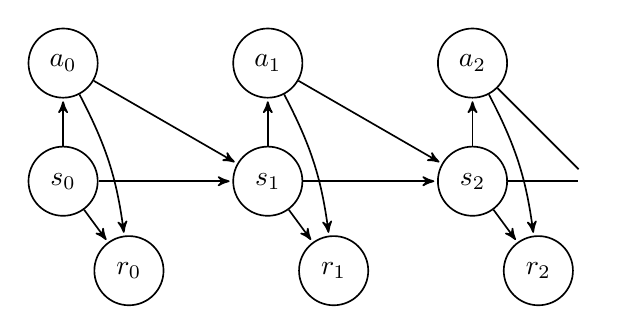
\begin{tikzpicture}[->,>=stealth',shorten >=1pt,auto,node distance=1.5cm,
                    semithick, baseline=1em]
	  \tikzstyle{every state}=[fill=white,draw=black,text=black]

	  \node[state] 		   (S0)                    	{$s_0$};
	  \node[state]         (S1) [right=1.7cm of S0] 		{$s_1$};
	  \node[state]         (S2) [right=1.7cm of S1] 		{$s_2$};

	  \node[state]         (A0) [above of=S0] 		{$a_0$};
	  \node[state]         (A1) [above of=S1]       {$a_1$};
	  \node[state]         (A2) [above of=S2]       {$a_2$};

	  \node[state]         (R0) [below right=0.5cm and 0.2cm of S0]	{$r_0$};
	  \node[state]         (R1) [below right=0.5cm and 0.2cm of S1]	{$r_1$};
	  \node[state]         (R2) [below right=0.5cm and 0.2cm of S2]	{$r_2$};

	  \node[]			(S3) [right of=S2] {};

	  \path (S0) edge (A0) edge (S1) edge (R0)
	  		(S1) edge (A1) edge (S2) edge (R1)
	  		(S2) edge (A2) edge[-] (S3) edge (R2)
	        (A0) edge[bend left=10] (R0) edge (S1)
	        (A1) edge[bend left=10] (R1) edge (S2)
	        (A2) edge[bend left=10] (R2)
	        (A2) edge[-] (S3);
	\end{tikzpicture}
\end{center}
\vspace{1em}

\noindent Da das gesamte System stochastischer Natur ist, lässt es sich mittels Wahrscheinlichkeitsverteilungen beschreiben. Es ist definiert durch
\begin{gather*}
	P(s_{0:T+1},a_{0:T},r_{0:T}; \pi)=\\P(s_0)\prod_{t=0}^TP(a_t|s_t;\pi)P(r_t|s_t,a_t)P(s_{t+1}|s_t,a_t).
\end{gather*}
Mit der initialen Zustandsverteilung $P(s_0)$, den Übergangsverteilungen $P(s_{t+1}|s_t,a_t)$, Verteilungen für den Reward $P(r_t|s_t,a_t)$ sowie der Policy des Agenten 
\begin{align*}
	\pi(a_t|s_t)&=P(a_0|s_0;\pi) &&\text{im stochastischen Fall, bzw.}\\
	a_t&=\pi(s_t)&&\text{deterministisch.}
\end{align*}%
In einem diskreten MDP können die Übergangswahrscheinlichkeiten $P(t_{t+1}|s_t,a_t)$ einfach als Tabelle gesehen werden.

Grundsätzlich wird angenommen, dass die Übergangs- und Rewardverteilungen unabgängig von der der Zeit sind und lediglich von Zustand und der getroffenen Aktion abhängen, diese Eigenschaft nennt man auch \emph{stationär}. 
Damit können wir die \emph{Rewardfunktion} sinnvoll definieren als
\begin{equation}\label{rewardfunction}
	R(s,a)\coloneqq\E\set{r}{s,a}=\int rP(r|s,a)\intd r.
\end{equation}

\paragraph{Zustandsbegriff in einem MDP}
Außerdem wichtig ist zu klären, was \enqo{Zustand} in einem MDP bedeutet. Wir definieren, dass für einen gegebenen Zustand die Vergangenheit konditional unabhängig von der Zukunft ist. Das heißt, alle möglichen \enqo{Zukünfte} $s_{t^+}$ für $t^+>t$ sind im Zustand $s_t$ kodiert. Oder allgemein
\begin{equation*}
	\forall t^+>t,t^-<t:\enspace\independent(s_{t^+},s_{t^-}|s_t).	
\end{equation*} 

\paragraph{Optimalität einer Policy}
Der \emph{Wert (Value)} eines Zustands $s$ beschreibt den erwarteten (discounted) reward bei einer Policy $\pi$, wenn in Zustand $s$ begonnen wird, das heißt
\begin{equation*}
 	V^\pi(s)\coloneqq\E\set{r_0+\gamma r_1+\gamma^2r_2+\ldots}{s_0=s;\pi}
 \end{equation*} 
mit Discounting-Faktor $\gamma\in[0,1]$. Das Discounting wird angewandt um Belohnungen in ferner Zukunft nur sehr klein zu bewerten.

Eine Policy $\pi^\ast$ ist optimal, wenn
\begin{equation*}
	\forall s:\enspace V^{\pi^\ast}(s)=V^\ast(s)\coloneqq\underset\pi\max\, V^\pi(s),
\end{equation*}
also gleichzeitig alle Values der möglichen Zustände maximiert werden.
In MDPs existiert immer mindestens eine optimale deterministische Policy.

\subsection{Valuefunktion}
Wir wollen noch einmal zurück zur Value-Funktion $V$ gehen und deren Eigenschaften betrachten. Sie ist ein zentrales Konzept in der gesamten Theorie des Reinforcement Lernens, denn viele Algorithmen lassen sich direkt aus ihr ableiten. Betrachten wir zunächst nur den Fall einer deterministischen Policy $\pi$, dann können wir die Valuefunktion rekursiv darstellen. Wir beginnen dazu mit der Definition
\begin{equation*}
	V^\pi(s)=\E\set{r_0+\gamma r_1+\gamma^2r_2+\ldots}{s_0=s;\pi}.
\end{equation*}
Den ersten Zustandsübergang und den damit einhergehenden Reward kann man nun herausziehen und erhält mit der Rewardfunktion aus \autoref{rewardfunction} dann
\begin{align*}
	V^\pi(s)&=\E\set{r_0}{s_0=s;\pi}\\
	&\quad+\gamma\E\set{r_1+\gamma r_2+\ldots}{s_0=s;\pi}\\
	&=R(s,\pi(s))\\
	&\quad+\gamma\sum_{s'}P(s'|s,\pi(s))\E\set{r_1+\ldots}{s_1=s';\pi}.
\end{align*}
Setzt man hier nun die Definition der Valuefunktion ein, erhält man die rekursive Darstellung
\begin{equation*}
	V^\pi(s)=R(s,\pi(s))+\gamma\sum_{s'}P(s'|s,\pi(s))V^\pi(s').
\end{equation*}
Der zweite Teil beschreibt den Wert/Value aller möglichen Folgezustände gewichtet mit den Wahrscheinlichkeiten der Übergänge.


Dies lässt sich genauso in Vektorschreibweise darstellen als
\begin{equation*}
	\mathbf V^\pi = \mathbf R^\pi+\gamma \mathbf P^\pi \mathbf V^\pi
\end{equation*}
mit den Vektoren $\mathbf V_s^\pi=V^\pi(s), \mathbf R_s^\pi=R(s,\pi(s))$ und der Wahrscheinlichkeitsmatrix $\mathbf P_{s,s'}^\pi=P(s'|s,\pi(s))$.

% \paragraph{Valuefunktion für stochastische Policies}
% Die rekursive Darstellung von $V$ für ein stochastisches $\pi(a|s)$ ist grundsätzlich analog
% \begin{equation*}
% 	V^\pi(s)=\sum_a\pi(a|s)R(s,a)+\gamma\sum_{s',a}\pi(a|s)P(s'|s,a)V^\pi(s').
% \end{equation*}

\subsubsection{Value Iteration}
Wir möchten nun einen ersten Ansatz finden, optimale Policies zu berechnen.
Wir verwenden dafür das Optimalitätsprinzip von Bellman, aus dem sich ergibt
\begin{equation*}
	V^\ast(s)=\max_a\bigg[R(s,a)+\gamma\sum_{s'}P(s'|s,a)V^\ast(s')\bigg].
\end{equation*}
Die zugehörige optimale Policy wählt immer die Aktion mit größtem erwarteten Reward, das heißt
\begin{equation*}
	\pi^\ast(s)=\underset a\argmax \bigg[R(s,a)+\gamma\sum_{s'}P(s'|s,a)V^\ast(s')\bigg].
\end{equation*}
Mit diesem Wissen lässt sich $V^\ast$ sinnvoll berechnen, das nachfolgende Verfahren ist die \emph{Value Iteration}.
Wir initialisieren $V_{k=0}(s)=0$. Dann berechnen wir für alle Zustände $s$ den Iterationsschritt
\begin{equation*}
	V_{k+1}(s)=\max_a\bigg[R(s,a)+\gamma\sum_{s'}P(s'|s,a)V_k(s')\bigg],
\end{equation*} 
bis das Abbruchkriterium
\begin{equation*}
	\max_s|V_{k+1}(s)<V_k(s)|\leq \epsilon
\end{equation*}
erreicht wird.
Die Valueiteration konvergiert gegen $V^\ast$.

\paragraph{Policy Evaluation}\label{policyEvaluation}
Anstatt eine optimale Valuefunktion zu berechnen, ist es natürlich genauso möglich die Valuefunktion $V^\pi$ einer gegebenen Policy $\pi$ zu berechnen. Dies funktioniert analog zur Value-Iteration mit dem Iterationsschritt
\begin{equation*}
	V_{k+1}^\pi(s)=R(s,\pi(s))+\gamma\sum_{s'}P(s'|s,\pi(s))V_k^\pi(s').
\end{equation*}
Genauso kann man auch die Matrixinversion
\begin{equation*}
	\mathbf V^\pi=(\mathbf I-\gamma\mathbf P^\pi)^{-1}\mathbf R^\pi
\end{equation*}
berechen.

\subsection{Q-Funktion}
Die Q-Funktion beziehungsweise \emph{State Action Value Function} gibt den Wert eines Zustands, gegeben der ersten ausgeführten Aktion an.
\begin{equation*}
	Q^\pi(s,a)=\E\set{r_0+\gamma r_1+\gamma^2 r_2+\ldots}{s_0=s,a_0=0;\pi}
\end{equation*}
Dies können wir analog zur Valuefunktion wieder rekursiv schreiben als
\begin{align*}
	Q^\pi(s,a)=R(s,a)+\gamma\sum_{s'}P(s'|s,a)Q^\pi(s',\pi(s')).
\end{align*}
Der Zusammenhang zur Valuefunktion ist
\begin{equation*}
	V^\pi(s)=Q^\pi(s,\pi(s))
\end{equation*}
beziehungsweise für die Valuefunktion bei optimalem Verhalten
\begin{align*}
	V^\ast(s)&=\max_aQ^\ast(s,a).
\end{align*}

\subsubsection{Q-Iteration}
Die Q-Iteration lässt sich vollkommen analog zur Value-Iteration schreiben. Es gilt 
\begin{align*}
	Q^\ast(s,a)=R(s,a)+\gamma\sum_{s'}P(s'\,|\,s,a)\max_{a'}Q^\ast (s',a'),
\end{align*}
womit wir wieder einen Algorithmus entwerfen.
Wir initialisieren $Q_0(s,a)=0$ für alle $s,a$.
Dann berechnen wir wiederum schrittweise für alle Kombinationen von Zuständen und Aktionen
\begin{equation*}
	Q_{k+1}(s,a)=R(s,a)+\gamma\sum_{s'}P(s'|s,a)\max_{a'}Q_{k}(s',a')
\end{equation*}
bis das Abbruchkriterium 
\begin{equation*}
	\max_{s,a}|Q_{k+1}(s,a)-Q_k(s,a)|\leq \epsilon
\end{equation*}
erreicht wird.
Die Q-Iteration konvergiert gegen $Q^\ast$.

\paragraph{Policy Iteration}
Man kann natürlich auch ein ähnliches iteratives Verfahren anwenden um die Policy $\pi$ schrittweise zu verbessern.
Wir initialisieren $\pi_0$ zum Beispiel zufällig.
Dann berechnen wir zunächst $Q^{\pi_k}$ (analog zu Policy Evaluation in \autoref{policyEvaluation}) und aktualisieren damit die Policy
\begin{equation*}
	\pi_{k+1}(s)=\underset a\argmax Q^{\pi_k}(s,a).
\end{equation*}
Dieses Verfahren heißt \emph{Policy Iteration}.



% \subsection{Belief State und Belief MDP}
% 05/24ff
% Kommen wir noch einmal zurück zum Banditenproblem, bisher haben wir Wissen dargestellt als die gesamte Historie der Entscheidungen und damit verbundenen Rewards
% \begin{equation*}
% 	h_t=[(a_1,y_1),(a_2,y_2),\ldots,(a_{t-1},y_{t-1})].
% \end{equation*}

% Aber dieses Wissen lässt sich noch auf eine andere Art und Weise darstellen. Der \emph{Belief} ist
% \begin{equation*}
% 	b_t(\theta)=P(\theta|h_t)
% \end{equation*}
% wobei $\theta=(\theta_1,\ldots,\theta_n)$ die unbekannten Parameter der Banditen sind.







\subsection{Partiell beobachtbare Markov-Entscheidungsprozesse (POMDP)}
Partiell beobachtbare Markov-Entscheidungsprozesse (partially observable markov decision processes, POMDPs) sind MDPs
4/22ff
7/11ff


















\section{Reinforcement Learning}
Bisher sind wir davon ausgegangen, die Welt zu kennen. Genauer heißt das, dass $P(s'|s,a)$ und $R(s,a)$ bekannt waren. Damit konnten wir mittels Value- bzw. Q-Iteration (also mit dynamischem Programmieren) optimale Policies bestimmen.

Wenn diese Werte bzw. Verteilungen nicht bekannt sind, befindet man sich im Themengebiet des reinforcement Lernens.
Ein mit der Welt interagierender Agent sammelt den Datensatz
\begin{equation*}
	D=\simpleset{(s_t,a_t,r_t,s_{t+1})}_{t=1}^T
\end{equation*}
und versucht daraus zu lernen.

Man muss hierbei unterscheiden, ob ein Modell der Welt bekannt ist oder nicht. Das heißt, ob ein Agent alle möglichen Zustände und Aktionen erfassen kann oder nicht. Je nachdem ob man modellbasiert oder modellfrei lernt sind die Lernansätze unterschiedlich.
\noindent
\begin{center}
	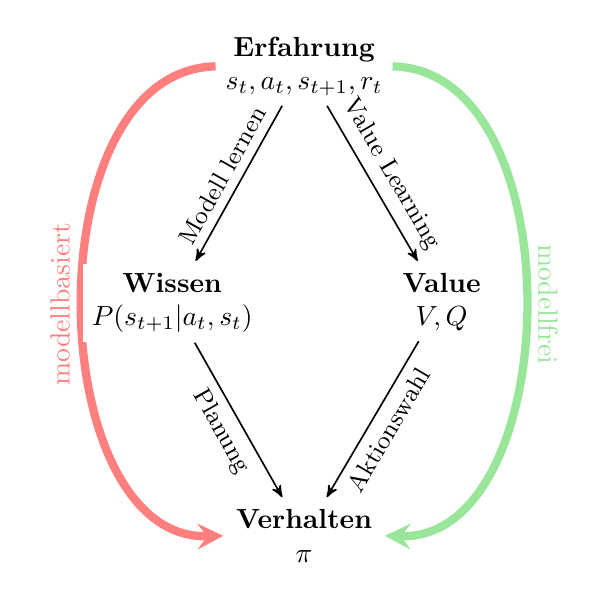
\begin{tikzpicture}[->,>=stealth',shorten >=1pt,auto,node distance=3.5cm,
                semithick, baseline=1em]
	  \tikzstyle{every state}=[fill=white,rectangle,draw=none,text=black,align=center]

	  \node[state] 		   (exp)                    	{\bf Erfahrung\\$\simpleset{s_t,a_t,s_{t+1},r_t}$};
	  \node[state]         (beh) [below=5cm of exp] 		{\bf Verhalten\\$\pi$};
	  
	  \begin{scope}[transparency group, opacity=0.5]
	  	\path (exp) edge[bend right=90,red,line width=3pt,-stealth] node[rotate=90,anchor=center,above]{modellbasiert} (beh);
	  	\path (exp) edge[bend left=90,green,line width=3pt,-stealth] node[rotate=-90,anchor=center,above]{modellfrei}(beh);
	  \end{scope}
	  


	  \node[state]         (kno) [below left=2cm and -0.6cm of exp] 		{\bf Wissen\\$P(s_{t+1}|a_t,s_t)$};
	  \node[state]         (val) [below right=2cm and 0cm of exp] 		{\bf Value\\$V,Q$};
	  

	  \path (exp) edge node[sloped, anchor=center, above]{\small Modell lernen} (kno) edge node[sloped, anchor=center, above]{\small Value Learning} (val)
	  (kno) edge node[sloped, anchor=center, below]{\small Planung} (beh)
	  (val) edge node[sloped, anchor=center, below]{\small Aktionswahl} (beh);
	  
	\end{tikzpicture}
\end{center}\noindent
Wir betrachten die genauen Unterschiede in den nachfolgenden Abschnitten.

\subsection{Modellfreies Reinforcement Learning}
Im modellfreien Reinforcement-Lernen sind die Übergangsverteilungen sowie die Rewards der Zustände unbekannt, es müssen nicht einmal alle Zustände bekannt werden. 
Ziel ist es zu lernen, den Value eines Zustands vorherzusagen. Das heißt die Algorithmen werden $V(s)$ bzw. $Q(s,a)$ schätzen.

\paragraph{On-Policy vs. Off-Policy Learning}
Es werden zwei Arten unterschieden. Ein On-Policy Lernverfahren lernt die Bewertung des Zustands und der Aktionen die von der Policy tatsächlich ausgeführt werden. Das heißt während der Agent $\pi$ ausführt wird auch $Q^\pi$ gelernt.

Ein Off-Policy-Verfahren hingegen lernt die optimale $Q$-Funktion $Q^\ast$ während eine \emph{beliebige} Policy $\pi$ ausgeführt wird. Die Policy wird lediglich zum Sammeln von Daten verwendet. Die Policy, nach der der Agent handelt ist nicht die gleiche wie die gelernte.


\subsubsection{Q-Learning}
Betrachten wir die Bellman-Optimalitätsgleichung für die $Q$-Funktion
\begin{equation*}
	Q^\ast(s,a)=R(s,a)+\gamma\sum_{s'}P(s'\,|\, s,a)\max_{a'}Q^\ast(s',a').
\end{equation*}
Wir möchten wieder basierend auf dieser Gleichung einen Algorithmus entwickeln der genauso wie die Q-Iteration ein $Q^\ast$ approximiert.
Doch ohne Modell der Welt kennen wir den zweiten Teil der Formel nicht, weder die möglichen Aktionen $a'$ noch die möglichen Zustände $s'$ sind bekannt.

Stattdessen lernen wir aus einzelnen Erfahrungen $(s,a,r,s')$ um so die $Q$-Funktion zu schätzen. Für jede Erfahrung berechnen wir basierend auf der vorherigen Q-Funktion die neue Approximation
\begin{align*}
	Q_{\text{new}}(s,a)&=(1-\alpha)Q_{\text{old}}(s,a)\\
	&\quad+\alpha[r+\gamma\max_{a'}Q_{\text{old}}(s',a')],
	\intertext{was wir weiter umformen zu}
	Q_{\text{new}}(s,a)&=Q_{\text{old}}(s,a)\\
	&\quad+\alpha\underbrace{[r+\gamma\max_{a'}Q_{\text{old}}(s',a')-Q_{\text{old}}(s,a)]}_{\text{TD error}}.
\end{align*}
So wird mit jedem Schritt der sogenannte \emph{temporal difference error} berechnet und als Korrekturfaktor addiert.
Ist der Reward $r$ größer als der erwartete Reward, das heißt
\begin{equation*}
	r>Q_{\text{old}}(s,a)-\gamma \max_{a'}Q_{\text{old}}(s',a'),
\end{equation*}
dann wird $Q_{\text{new}}(s,a)$ erhöht. Analog wird der Wert verringert, wenn $r$ kleiner als die Erwartung ist.
Dieses Verfahren wird \emph{Q-Learning} genannt, es ist ein Off-Policy-Lernalgorithmus.

Besonders bemerkenswert ist, dass eine mit Q-Learning gelernte Q-Funktion beweisbar gegen $Q^\ast$ konvergiert. Für den Beweis wurde lediglich die \emph{mixing property} angenommen. Das heißt, dass es von jedem Zustand aus eine Wahrscheinlichkeit $>0$ gibt in jeden anderen Zustand zu gelangen.

Ein Pseudocode des Q-Learning-Algorithmus sieht dann wie folgt aus.
\begin{lstlisting}
(*$Q(s,a)=0$*)
while unhappy
	initialize start state (*$s$*)
	while in episode
		Choose action (*$a\approx_\epsilon\underset a\argmax Q(s,a)$*)
		Take action (*$a$*), observe (*$r,s'$*)
		(*$Q(s,a)\leftarrow Q(s,a)+\alpha[r+\gamma\max_{a'}Q(s',a')-Q(s,a)]$*)
		(*$s\leftarrow s'$*)
	end
end\end{lstlisting}
Hierbei wurde die sogenannte \emph{epsilon greedy}-Strategie ($\approx_\epsilon$) verwendet. Das bedeutet lediglich, dass mit Wahrscheinlichkeit $\epsilon$ eine zufällige Aktion gewählt wird und nur mit Wahrscheinlichkeit $1-\epsilon$ tatsächlich das gewünschte $\argmax$. In Formel also
\begin{gather*}
	a\approx_\epsilon \underset a\argmax Q(s,a)\Longleftrightarrow\\ a=\begin{cases}
		\text{random},&\text{Wahrscheinlichkeit }\epsilon\\
		\underset a\argmax Q(s,a),&\text{sonst.}
	\end{cases}
\end{gather*}
Damit wird sichergestellt, dass der Algorithmus genügend exploriert und neue Daten sammelt, also eben nicht immer die optimale Aktion ausführt. Somit werden zum Beispiel lokale Maxima vermieden.

Desweiteren wird der Algorithmus in sogenannten Episoden ausgeführt, nach denen jedes mal der Startzustand wiederhergestellt wird bevor der Agent weiter agieren kann. Oft ist die Anzahl der auszuführenden Schritte in einer Episode festgelegt. Episoden stellen sicher, dass der Agent nicht in non-return areas gefangen bleibt und Lernen für immer verhindert wird (Klippe heruntergefallen, Objekt mit dem interagiert wird ist kaputt,\ldots).

\subsubsection{Varianten des Q-Learning}
Es gibt viele Varianten des Basis-Q-Learning. Sie
\paragraph{Eligibility Traces}
Bisher sind die Lernverfahren sehr langsam, da ein erzielter Reward immer nur einen Schritt \enqo{in die Vergangenheit} weitergereicht wird.
Aber alle Zustände entlang eines Pfads, der zu einem Erfolg führt, sollten aktualisiert werden. Erhält einen Reward, ist nicht nur die letzte getroffene Entscheidung die entscheidende Aktion, sondern der gesamte gegangene Pfad ist wichtig.
\emph{Eligibility Traces} bewerten (mit Discounting und Skalierungsfaktor) den gesamten Pfad so wird aus der gesamten Vergangenheit bis zum Reward gelernt. Die $Q$-Tabelle wird viel schneller gefüllt und damit schneller gelernt.


\paragraph{TD}
Der \emph{Temporal Difference}-Lernalgorithmus lernt aus der Erfahrung $(s,r,s')$, indem die Valuefunktion im Zustand $s$ durch
\begin{equation*}
	V(s)\leftarrow V(s)+\alpha [r+\gamma V_{\text{old}}(s')-V_{\text{old}}(s)]
\end{equation*}
aktualisiert wird.

Mit Verwendung von einer längeren Historie kann man ganze Erfahrungssequenzen mit einbeziehen, zum Beispiel $(s_0,r_0,r_1,r_2,s_3)$ und damit
\begin{equation*}
	V(s_0)\leftarrow V(s_0)+\alpha [r_0+\gamma r_1+\gamma^2r_2+\gamma^3 V_{\text{old}}(s_3)-V_{\text{old}}(s_0)]
\end{equation*}
berechnen. Dies nennt man dann \emph{Temporal Credit Assignment}.

Bei den beiden Verfahren wurde bisher immer nur ein Zustand aktualisiert, wir betrachten nun den $\mathrm{TD}(\lambda)$-Algorithmus, der Eligibility auf elegante Art und Weise unterbringt und damit mit einer Erfahrungssequenz mehrere Zustände aktualisieren kann.

Die Eligibility-Funktion wird immer beim Besuchen des Zustands $s_t$ aktualisiert
\begin{equation*}
	e(s_t)\leftarrow e(s_t)+1.
\end{equation*}
Die Funktion \enqo{merkt sich}, dass der Zustand vor kurzem besucht wurde. Unter Verwendung dieser Funktion wird dann die Valuefunktion aktualisiert
\begin{equation*}
	\forall s:V(s)\leftarrow V(s)+\alpha e(s)*[r_t+\gamma V(s_{t+1})-V(s_t)].
\end{equation*}
Wichtig ist hierbei, dass alle Zustände aktualisiert werden.
Zustände die nicht oder lange nicht mehr besucht wurden haben dabei einen kleinen Eligibility-Wert, da man in jedem Schritt das Discounting
\begin{equation*}
	\forall s:e(s)\leftarrow \gamma\lambda e(s)
\end{equation*}
anwendet.

\paragraph{SARSA}
SARSA verwendet die Erfahrung $(s,a,r,s',a')$ um die $Q^\pi$-Funktion zu schätzen. Dabei wird auch wieder die Eligibility $e(s)$ genauso wie oben bereits angesprochen verwendet.
\begin{align*}
	\forall s,a:Q(s,a)&\leftarrow Q(s,a)+\alpha e(s,a)*\\
	&\quad[r+\gamma Q_{\text{old}}(s',a')-Q_{\text{old}}(s,a)]
\end{align*}

\paragraph{$Q(\lambda)$}
Das $Q(\lambda)$-Verfahren stellt \emph{das} Verfahren für $Q$-Learning dar, da es von den besprochenen das einzige ist, dass $Q^\ast$ beim Ausführen einer beliebigen Policy ist. $Q(\lambda)$ ist also ein Off-Policy Lernverfahren.
Mit der Eligibility $e(s)$ wird in jedem Schritt 
\begin{align*}
	\forall s,a:Q(s,a)&\leftarrow Q(s,a)+\alpha e(s,a)*\\
	&\quad[r+\gamma \max_{a'} Q_{\text{old}}(s',a')-Q_{\text{old}}(s,a)]
\end{align*}
aktualisiert.





\paragraph{Experience Replay}
In einem großen Zustandsraum kann es schwierig sein eine gesamte $e(s,a)$-Tabelle zu speichern und die Aktualisierung für alle $s,a$ auszuführen. Daher wird hier oft ein \emph{replay buffer}
\begin{equation*}
	D=\simpleset{(s_i,a_i,r_i,s_{i+1})}_{i=0}^t
\end{equation*}
im Zeitpunkt $t$ gespeichert. Nun wird in jedem Schritt für eine Teilmenge $B\subseteq D$ und die neueste Erfahrung die $Q$-Funktion aktualisiert
\begin{equation*}
	Q(s,a)\leftarrow Q(s,a)+\alpha*[r+\gamma\max_{a'}Q(s',a')-Q(s,a)].
\end{equation*}
Dies nennt man \emph{Experience Replay}.

\subsection{Modellbasiertes Reinforcement Learning}
Im modellbasierten Reinforcement Learning sind Dinge wie Wissen (das über Values hinaus geht), Planung und Antizipation der nächsten Zustände unmöglich.
Beziehungsweise, noch viel extremer, wenn sich das Ziel ändert, muss der Agent wieder von vorne beginnen, da sich alle bereits gelernten Werte ändern.




Der Agent wird dann versuchen
\begin{itemize}
	\item den nächsten Zustand vorherzusagen, genauer $P(s'|s,a)$ und
	\item den zugehörigen Reward, also $P(r|s,a)$ zu schätzen.
\end{itemize}







todo


\begin{itemize}
	\item Belief State
	\item Lernen in MDPs, modellbasiert/modellfrei
	\item Diskussion Grenzen von modellfreiem Lernen 
	\item R-MAX
\end{itemize}




\subsection{Q-learning} Folie 11/50



Aus den neuen Erfahrungen die Zustände und Aktionen zu bewerten ist Reinforcement Learning

Schätzen und mit Lernrate $\alpha$ langsam annähern. Ohne Lernrate ist der Teil nach $\alpha$ zu stochastisch verrauscht. Neue Schätzung mit Low-Pass-Filter versehen. Lernen aus einer einzigen Erfahrung.

R(s,a): Erwartungswert der sofortigen Belohnung wenn ich Aktion a in Zustand s ausführe

Q-Funktion: Wie viel 

V-Funktion: $V^\pi(s)$ Return den ich erwarte wenn ich Policy $\pi$ benutze. $V^\ast$ optimales Verhalten









%!TEX root=main.tex
\section{Constraint Satisfaction Probleme}
Eine Variablenbelegung unter bestimmten Bedingungen zu finden ist ein fundamentales Problem. \emph{Constraint Satisfaction Probleme (CSP)} formalisieren diese Problemstellung.
\begin{definition}[Constraint Satisfaction Problem]
	Ein \emph{Constraint Satisfaction Problem (CSP)} besteht aus $n$ Variablen $X_i$ mit zugehörigen \emph{Domains} $D_i, x_i\in D_i$ und $K$ \emph{Constraints} $C_k$.
	Jedes Constraint trifft eine Aussage über die Belegung einer Teilmenge aller Constraints. Genauer ist ein Constraint $C_k$ ein Tupel $C_k=(I_k,c_k)$ wobei $I_k\subseteq\simpleset{1,\ldots,n}$ die Teilmenge der betroffenen Variablen ist. Die Abbildung $c_k:D_{I_k}\rightarrow \simpleset{0,1}$ bestimmt, ob die Konfiguration der $x_{I_k}\in D_{I_k}$ zulässig ist.

	Das Ziel ist, eine Konfiguration $X=(X_1,\ldots,X_n)$ aller Variablen zu finden, sodass alle Constraints erfüllt sind.
\end{definition}

Ein CSP lässt sich als \emph{Constraint Graph} darstellen. Dies ist ein bipartiter Graph, in dem Variablen als Kreise und Constraints als Kästen dargestellt werden. Ein Beispiel ist der nachfolgende Constraintgraph.
\noindent
\begin{center}
	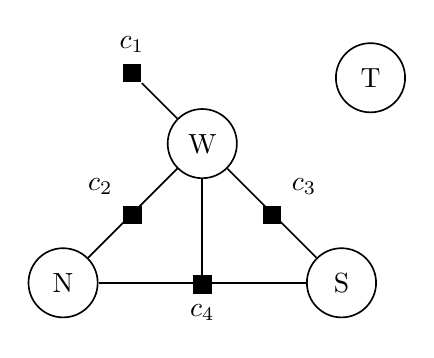
\begin{tikzpicture}[auto,node distance=2.5cm,semithick, baseline=1em]
	  \tikzstyle{every state}=[fill=white,circle,draw=black,text=black,align=center]

	  \node[state] (W) {W};
	  \node[state] (N) [below left of=W] {N};
	  \node[state] (S) [below right of=W] {S};
	  \node[state] (T) [above right=0.2cm and 1.5cm of W] {T};

	  \path (W) edge node[rectangle, fill=black, label={above left:$c_2$},below=-3pt]{} (N)
	  (N) edge node[rectangle, fill=black, label={below:$c_4$},below=-3pt]{} (S)
	  (W) edge node[rectangle, fill=black, label={above right:$c_3$},below=-3pt]{} (S)
	  node[rectangle, fill=black, label={above:$c_1$},above left=0.45cm and 0.45cm of W]{} edge (W)
	  node[below=1.4cm of W] {} edge (W);
	\end{tikzpicture}
\end{center}
\noindent
Das zugehörige CSP hat 4 Variablen und ebenfalls 4 Constaints. Man sieht, dass die Constraints unterschiedliche Anzahlen an Variablen beeinflussen können.
Es gilt $I_1=\simpleset{W},I_2=\simpleset{W,N},I_3=\simpleset{W,S}$ und $I_4=\simpleset{N,W,S}$. Auch möglich ist, dass eine Variable von keinem Constraint beeinflusst wird, wie an $T$ zu sehen.
\begin{itemize}
	\item $C_1$ ist ein sogenanntes \emph{unäres Constraint}, da $|I_1|=1$.
	Ein Beispiel wäre $W\neq \text{rot}$.
	\item Die Constraints $C_2,C_3$ sind \emph{binäre Constraints}, da $|I_2|=|I_3|=2$. Ein Beispiel wäre $W\neq N$.
	\item Und das Constraint $I_4$ ist ein \emph{Constraint höherer Ordnung}, da $|I_4|>2$.
\end{itemize}

Sind alle Domainräume endlich und haben die gleiche Größe $d=|D_i|$, dann ist der Aufwand das CSP zu lösen in $\mathcal O(d^n)$.

\subsection{Lösen eines diskreten CSP}
Der \enqo{brute force} Lösungsalgorithmus für ein CSP ist \emph{sequential assignment}. Der Algorithmus weist Variablen Werte zu, solange dies nicht den Constraints widerspricht. Implementiert wird dies als eine Tiefensuche in einem Baum mit branching factor $(n-l)d$ bei Tiefe $l$. Der Baum hat also $n!d^n$ Blätter!

Eine erste Verbesserung dieses Algorithmus ist \emph{Backtracking Sequential Assignment}. Die entscheidende Erkenntnis ist, dass es für die Vollständigkeit des Algorithmus keine Rolle spielt in welcher Reihenfolge die Variablen gesetzt werden.
Insbesondere kann man also eine Reihenfolge festlegen und damit den branching factor des Baums drastisch reduzieren. In jeder Tiefe ist der der branching factor $d$, was nur noch $d^n$ Blätter zu Folge hat.
Hiermit erreicht man den oben angesprochenen Zeitaufwand von $\mathcal O(d^n)$.

08/13
\begin{lstlisting}
function backtrackingSearch(csp)
	return recBacktracking({}, csp)
end

function recBacktracking(assignment, csp)
	if assignment.isComplete then return assignment
	var = selectUnassignedVariable(variables(csp), assignment, csp)
	for value in orderedDomainValues(var, assignment, csp) do
		if value consistent with assignment given constraints(csp) then
			add [var = value] to assignment
			result = recursiveBacktracking(assignment, csp)
			if result != failure then return result
			remove [var = value] from assignment
		end
	end
	return failure
end
\end{lstlisting}

\subsection{Möglichkeiten der Verbesserung}
Mithilfe von simplen Heuristiken kann man die Laufzeit des Lösungsalgorithmus stark verringern. Dabei gibt es mehrere Angriffspunkte zur Optimierung, wir betrachten zunächst welche Variable am besten als nächstes zur Belegung gewählt werden sollte sowie die Reihenfolge der Wertebelegungen.
\subsubsection{Variablenreihenfolge}
Mit der \emph{Minimum remaining Values (MRV)}-Heuristik kann man die Breite des Baums stark verringern. Wir wählen die Variable, der als nächstes ein Wert zugewiesen werden soll so, dass sie die wenigsten möglichen Wertebelegungen hat. So ist der branching factor des Baums zu Beginn klein.

Hier können natürlich Fälle auftreten, bei denen diese Entscheidung nicht eindeutig ist. Wir führen die \emph{Degree Heuristic} als Tie Breaker ein. Hier wird immer die Variable als nächstes gewählt, die die meisten Constrains auf noch unbelegte Variablen hat. Damit werden gleichzeitig die möglichen Wertebelegungen der bisher unbelegten Variablen verringert.

\subsubsection{Wertereihenfolge}
Sind bei einer Variablenbelegung mehrere Werte möglich wählt man mit der \emph{Least Constraining Value}-Heuristik immer den Wert, der noch die meisten Wertebelegungen bei den noch unbelegten Variablen zulässt.

\subsubsection{Inferenz}
Mit den bisher besprochenen Optimierungen ist nicht alles abgedeckt. Durch Anwenden von Inferenz können wir frühzeitig feststellen ob eine Lösung überhaupt noch möglich ist, was natürlich bedeutet dass wir das Backtracking früher beginnen können.
\paragraph{Constraint Propagation}
Nach jeder Wertezuweisung können die möglichen Belegungen der übrigen Variablen berechnet werden. Das heißt nach jeder Zuweisung werden aus den Domains $D_i$ entsprechend den Constraints alle nicht mehr möglichen Werte entfernt. Dies kann rekursiv geschehen, da das Löschen eines Werts wiederum die Domains beeinflussen kann.
Diese Denkweise ist \emph{Inferenz}. Das angewandte Verfahren heißt \emph{Constraint Propagation}, da wir implizite Constraints propagieren und so die Domains verkleinern.

Für binäre Constraints wird Constraint Propagation auch \emph{Arc Consistency} genannt.

Betrachten wir ein kleines Beispiel. Die nachfolgenden Variablen haben alle den gleichen Domainraum $D=\simpleset{\text{\color{red}rot},\text{\color{blue}blau},\text{\color{green}grün}}$. Alle Constraints fordern, wie im Constraintgraph eingetragen, Ungleichheit der Variablen. Es handelt sich hier also um ein Färbungsproblem. Die Domains wurden in die Nähe der Variablen eingetragen.
\noindent
\begin{center}
	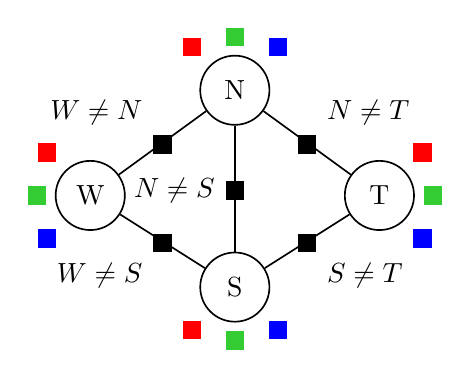
\begin{tikzpicture}[auto,node distance=2.5cm,semithick, baseline=1em]
	  \tikzstyle{every state}=[fill=white,circle,draw=black,text=black,align=center]
	  \tikzstyle{constraint}=[rectangle, fill=black, below=-3pt]

	  \node[state] (N) {N};
	  \node[state] (W) [below left=0.7cm and 1.2cm of N] {W};
	  \node[state] (S) [below of=N] {S};
	  \node[state] (T) [below right=0.7cm and 1.2cm of N] {T};

	  \path 
	  (N) edge node[constraint, label={above left:$W\neq N$},below=-3pt]{} (W)
	  edge node[constraint, label={above right:$N\neq T$}] {} (T)
	  

	  (S) edge node[constraint, label={below right:$S\neq T$}] {} (T)
	  edge node[constraint, label={left:$N\neq S$}]{} (N)
	  edge node[constraint, label={below left:$W\neq S$}]{} (W)
	  ;

	  \node[constraint] [fill=red,above left=0.1cm and 0.1cm of N] {};
	  \node[constraint] [fill=green,above=0.1cm of N] {};
	  \node[constraint] [fill=blue,above right=0.1cm and 0.1cm of N] {};

	  \node[constraint] [fill=red,above left=0.1cm and 0.1cm of W] {};
	  \node[constraint] [fill=green,left=0.1cm of W] {};
	  \node[constraint] [fill=blue,below left=0.1cm and 0.1cm of W] {};

	  \node[constraint] [fill=red,below left=0.1cm and 0.1cm of S] {};
	  \node[constraint] [fill=green,below=0.1cm of S] {};
	  \node[constraint] [fill=blue,below right=0.1cm and 0.1cm of S] {};

	  \node[constraint] [fill=red,above right=0.1cm and 0.1cm of T] {};
	  \node[constraint] [fill=green,right=0.1cm of T] {};
	  \node[constraint] [fill=blue,below right=0.1cm and 0.1cm of T] {};
	\end{tikzpicture}
\end{center}
\noindent
Färben wir zu erst $W$ rot, sehen wir dass sich die Domains anpassen.
\noindent
\begin{center}
	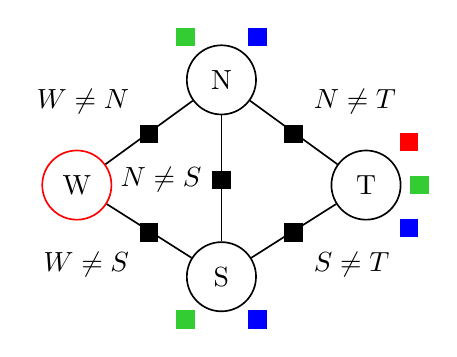
\begin{tikzpicture}[auto,node distance=2.5cm,semithick, baseline=1em]
	  \tikzstyle{every state}=[fill=white,circle,draw=black,text=black,align=center]
	  \tikzstyle{constraint}=[rectangle, fill=black, below=-3pt]

	  \node[state] (N) {N};
	  \node[state] (W) [draw=red,below left=0.7cm and 1.2cm of N] {W};
	  \node[state] (S) [below of=N] {S};
	  \node[state] (T) [below right=0.7cm and 1.2cm of N] {T};

	  \path 
	  (N) edge node[constraint, label={above left:$W\neq N$},below=-3pt]{} (W)
	  edge node[constraint, label={above right:$N\neq T$}] {} (T)

	  (S) edge node[constraint, label={below right:$S\neq T$}] {} (T)
	  edge node[constraint, label={left:$N\neq S$}]{} (N)
	  edge node[constraint, label={below left:$W\neq S$}]{} (W)
	  ;

	  \node[constraint] [fill=green,above left=0.1cm and 0.01cm of N] {};
	  \node[constraint] [fill=blue,above right=0.1cm and 0.01cm of N] {};

	  \node[constraint] [fill=green,below left=0.1cm and 0.01cm of S] {};
	  \node[constraint] [fill=blue,below right=0.1cm and 0.01cm of S] {};

	  \node[constraint] [fill=red,above right=0.1cm and 0.1cm of T] {};
	  \node[constraint] [fill=green,right=0.1cm of T] {};
	  \node[constraint] [fill=blue,below right=0.1cm and 0.1cm of T] {};
	\end{tikzpicture}
\end{center}
\noindent
Legen wir nun noch $T$ auf grün fest.
\noindent
\begin{center}
	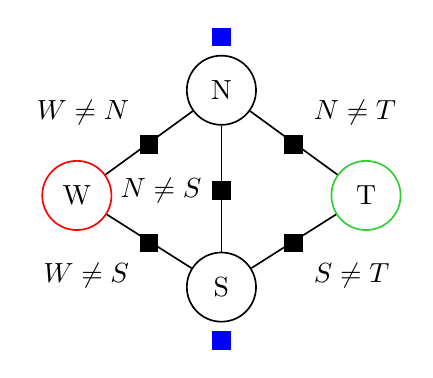
\begin{tikzpicture}[auto,node distance=2.5cm,semithick, baseline=1em]
	  \tikzstyle{every state}=[fill=white,circle,draw=black,text=black,align=center]
	  \tikzstyle{constraint}=[rectangle, fill=black, below=-3pt]

	  \node[state] (N) {N};
	  \node[state] (W) [draw=red,below left=0.7cm and 1.2cm of N] {W};
	  \node[state] (S) [below of=N] {S};
	  \node[state] (T) [draw=green,below right=0.7cm and 1.2cm of N] {T};

	  \path 
	  (N) edge node[constraint, label={above left:$W\neq N$},below=-3pt]{} (W)
	  edge node[constraint, label={above right:$N\neq T$}] {} (T)

	  (S) edge node[constraint, label={below right:$S\neq T$}] {} (T)
	  edge node[constraint, label={left:$N\neq S$}]{} (N)
	  edge node[constraint, label={below left:$W\neq S$}]{} (W)
	  ;

	  \node[constraint] [fill=blue,above=0.1cm of N] {};

	  \node[constraint] [fill=blue,below=0.1cm of S] {};
	\end{tikzpicture}
\end{center}
\noindent
Man würde hier bereits nach zwei Schritten sehen, dass für $N$ und $S$ jeweils nur noch ein Wert möglich ist $D_N=D_S=\simpleset{{\color{blue}\text{blau}}}$. Aber die beiden Variablen dürfen wegen dem $N\neq S$ Constraint nicht mit dem selben Wert belegt werden.

Man kann Konsistenz nach \emph{arc consistency} formalisieren, als ein Constraint $X\rightarrow Y$ heißt konsistent, wenn für jeden Wert $x$ von $X$ ein erlaubter Wert $y$ existiert.

\subsection{CSPs in Baumstruktur}
Hat der Constraintgraph eine Baumstruktur, so kann man das CSP in $\mathcal O(nd^2)$ lösen. Da dieser Aufwand so viel kleiner ist als $\mathcal O(d^n)$ eines allgemeinen CSP gibt es viele Algorithmen die versuchen ein CSP zu lösen indem es schrittweise in Baumstruktur gebracht wird.

Zunächst betrachten wir den Lösungsalgorithmus für baumstrukturierte CSP. Man wählt eine Variable als Wurzel, und ordnet alle anderen Variablen so an, dass Kindknoten immer nach ihren Eltern eingeordnet werden.
Zum Beispiel könnten die Variablen dieses Constraintgraphen folgendermaßen angeordnet werden.
\noindent
\begin{center}
	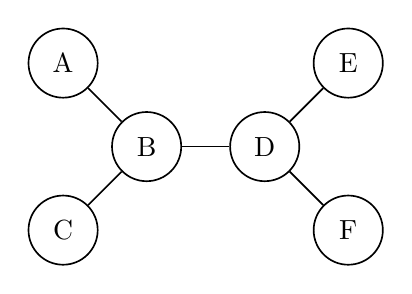
\begin{tikzpicture}[-,auto,node distance=1.5cm,
                    semithick, baseline=1em]
	  \tikzstyle{every state}=[fill=white,draw=black,text=black]

	  \node[state]         (B)  		{B};
	  \node[state] 		   (A) [above left of=B]        {A};
	  \node[state]         (C) [below left of=B] 		{C};

	  \node[state]         (D) [right of=B] 		{D};
	  \node[state]         (E) [above right of=D]       {E};
	  \node[state]         (F) [below right of=D]       {F};

	  \path (B) edge (A) edge (C) edge (D)
	  (D) edge (E) edge (F);
	\end{tikzpicture}

	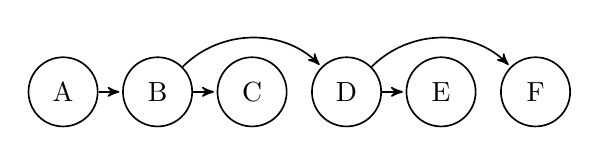
\begin{tikzpicture}[->,>=stealth',shorten >=1pt,auto,node distance=1.2cm,
                    semithick, baseline=1em]
	  \tikzstyle{every state}=[fill=white,draw=black,text=black]

	  \node[state] 		   (A)         {A};
	  \node[state]         (B) [right of=A] 		{B};
	  \node[state]         (C) [right of=B] 		{C};

	  \node[state]         (D) [right of=C] 		{D};
	  \node[state]         (E) [right of=D]       {E};
	  \node[state]         (F) [right of=E]       {F};

	  \path (A) edge (B)
	  (B) edge (C) edge[in=135, out=45] (D)
	  (D) edge (E) edge[in=135, out=45] (F);
	\end{tikzpicture}
\end{center}
\noindent
Anschließend wird über diese Anordnung iteriert.
Von den Blättern zur Wurzel, d.h. für $j$ von $n$ bis $2$ werden alle Wertebelegungen aus $D_{\mathrm{Parent}(X_j)}$ gelöscht, die nicht konsistent mit dem Constraint zwischen $X_j$ und seinem Elternknoten sind.
Anschließend können von der Wurzel zu den Blättern hin Werte zugewiesen werden.
Das heißt für $j$ von $1$ bis $n$ wird $X_j$ ein Wert zugewiesen, der konsistent mit der Belegung von $\mathrm{Parent}(X_j)$ ist.
Nach der Definition von Konsistenz muss es für jede noch mögliche Belegung des Elternknotens mindestens eine Belegung von $X_j$ geben.

Wir wissen nun, dass man solche CSPs einfach lösen kann und möchten dies auf allgemeinere CSPs anwenden.

Ein baumähnliches CSP kann man \emph{konditionieren}. Dafür werden einige Variablen belegt, bis der übrige Graph ein Baum ist. Dabei müssen wir natürlich die Domains der Nachbarn der belegten Variablen entsprechend anpassen. Betrachten wir den Constraintgraphen
\noindent
\begin{center}
	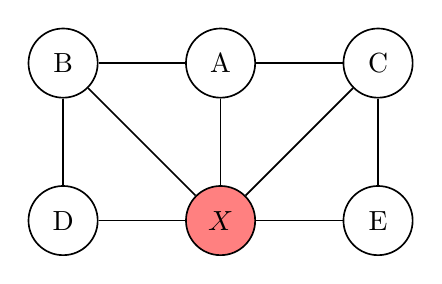
\begin{tikzpicture}[auto,node distance=2cm,semithick, baseline=1em]
	  \tikzstyle{every state}=[fill=white,circle,draw=black,text=black,align=center]
	  \tikzstyle{constraint}=[rectangle, fill=black, below=-3pt]

	  \node[state] (N) {A};
	  \node[state] (S) [fill=red!50!white, below of=N] {$X$};
	  \node[state] (W) [left of=N] {B};
	  \node[state] (Q) [right of=N] {C};
	  \node[state] (E) [below of=Q] {E};
	  \node[state] (V) [below of=W] {D};

	  \path (S) edge (W) edge (N) edge (Q) edge (E) edge (V)
	  (V) edge (W)
	  (W) edge (N)
	  (N) edge (Q)
	  (Q) edge (E);
	\end{tikzpicture}
\end{center}
\noindent
Durch Entfernen von $X$ bleibt ein Baum übrig. Durch Verwenden dieses Verfahrens kann, bei $c$ \enqo{abgeschnittenen} Variablen eine Laufzeit in $\mathcal O(d^c*(d-c)d^2)$ erreicht werden, was besonders für kleine $c$ sehr gut ist.











\section{Graphische Modelle von probabilistischen Systemen}











Unabhängigkeit von Zufallsvariablen sollte klar sein, wir haben wir diese Eigenschaft streng genommen sogar bereits benutzt, der Vollständigkeit halber definieren wir sie hier noch einmal.
\begin{definition}[Unabhängigkeit]
	Zwei Zufallsvariablen $X,Y$ heißen \emph{unabhängig}, wenn
	\begin{equation*}
		\independent(X,Y)\Longleftrightarrow P(X,Y)=P(X)*P(Y)
	\end{equation*}
	gilt. Analog sind sie \emph{konditional unabhängig}, wenn
	\begin{equation*}
		\independent(X,Y|Z)\Longleftrightarrow P(X,Y|Z)=P(X|Z)*P(Y|Z).
	\end{equation*}
\end{definition}


\subsection{Bayesnetze}
09/*ff



\begin{definition}[Bayesnetz]
	Ein \emph{Bayesnetz} ist ein gerichteter azyklischer Graph, bei dem jeder Knoten eine Zufallsvariable repräsentiert. Für jeden Knoten $X_i$ gibt es eine konditionale Wahrscheinlichkeitsverteilung für dessen Wert
	\begin{equation*}
		P(X_i\,|\,\mathrm{Parents}(X_i)).
	\end{equation*}
	Üblicherweise stellt man beobachtete Variablen d.h. Variablen, deren Werte bekannt sind, mit grauer Schattierung dar.
\end{definition}
Die gemeinsame Verteilung kann man durch
\begin{equation*}
	P(X_{1:n})=\prod_{i=1}^nP(X_i\,|\,\mathrm{Parents}(X_i))
\end{equation*}
faktorisieren. Wobei $\mathrm{Parents}(X_i)$ die Vorgänger von $X_i$ sind, d.h. ein Knoten $v\in\mathrm{Parents}(X_i)$ genau dann, wenn eine Kante $(v,X_i)$ im Bayesnetz existiert.

Um Unabhängigkeit von Variablen in Bayesnetzen zu entscheiden gibt es grundsätzlich drei Fälle, die eine Hilfe sein können.
\begin{enumerate}
	\item Head to Head:
	\begin{center}
		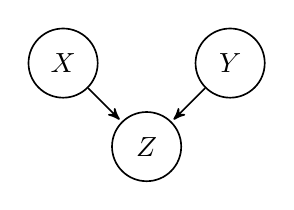
\begin{tikzpicture}[->,>=stealth',shorten >=1pt,auto,node distance=1.5cm,
	                    semithick, baseline=1em]
		  \tikzstyle{every state}=[fill=white,draw=black,text=black,text width=0.5cm, align=center]

		  \node[state] 		   (X)                    	{$X$};
		  \node[state]         (Z) [below right of=X] 		{$Z$};
		  \node[state]         (Y) [above right of=Z] 		{$Y$};

		  \path (X) edge (Z)
		  (Y) edge (Z);
		\end{tikzpicture}
	\end{center}
	Es gilt $\independent(X,Y)$ und $\neg\independent(X,Y|Z)$, denn
	\begin{align*}
		P(X,Y,Z)&=P(X)P(Y)P(Z|X,Y)\\
		P(X,Y)&=P(X)P(Y)\sum_ZP(Z|X,Y)\\
		&=P(X)P(Y).
	\end{align*}

\item Tail to Tail:
	\begin{center}
		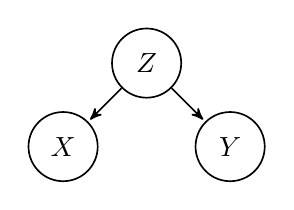
\begin{tikzpicture}[->,>=stealth',shorten >=1pt,auto,node distance=1.5cm,
	                    semithick, baseline=1em]
		  \tikzstyle{every state}=[fill=white,draw=black,text=black,text width=0.5cm, align=center]

		  \node[state] 		   (X)                    	{$X$};
		  \node[state]         (Z) [above right of=X] 		{$Z$};
		  \node[state]         (Y) [below right of=Z] 		{$Y$};

		  \path (Z) edge (X) edge (Y);
		\end{tikzpicture}
	\end{center}
	Es gilt $\neg\independent(X,Y)$ und $\independent(X,Y|Z)$, denn
	\begin{align*}
		P(X,Y,Z)&=P(Z)P(X|Z)P(Y|Z)\\
		P(X,Y|Z)&=\frac{P(X,Y,Z)}{P(Z)}\\
		&=P(X|Z)P(Y|Z).
	\end{align*}

\item Head to Tail:
	\begin{center}
		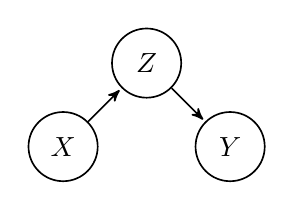
\begin{tikzpicture}[->,>=stealth',shorten >=1pt,auto,node distance=1.5cm,
	                    semithick, baseline=1em]
		  \tikzstyle{every state}=[fill=white,draw=black,text=black,text width=0.5cm, align=center]

		  \node[state] 		   (X)                    	{$X$};
		  \node[state]         (Z) [above right of=X] 		{$Z$};
		  \node[state]         (Y) [below right of=Z] 		{$Y$};

		  \path (X) edge (Z) 
		  (Z) edge (Y);
		\end{tikzpicture}
	\end{center}
	Es gilt $\neg\independent(X,Y)$ und $\independent(X,Y|Z)$, denn
	\begin{align*}
		P(X,Y,Z)&=P(X)P(Z|X)P(Y|Z)\\
		P(X,Y|Z)&=\frac{P(X,Y,Z)}{P(Z)}=\frac{P(X,Z)P(Y|Z)}{P(Z)}\\
		&=P(X|Z)P(Y|Z).
	\end{align*}

\end{enumerate}



\subsection{Inferenz in graphischen Modellen}
In Bayesnetzen können wir genauso Inferenz betreiben und aus Informationen der beobachteten Variablen oder a priori-Informationen Aussagen über andere Variablen treffen.

\subsubsection{Variablenelimination}
\begin{enumerate}
	\item Variablenelimination
	\item Faktorgraphen
	\item Message Passing
	\item Loopy belief propagation
	\item Sampling Methods?
\end{enumerate}

\subsection{Decision Making}
\subsection{Learning}
\subsection{Structure Learning}

\section{Dynamische Modelle}
\subsection{Markovprozesse und -ketten}
Markovprozess erster Ordnung
\vspace{1em}
\noindent
\begin{center}
	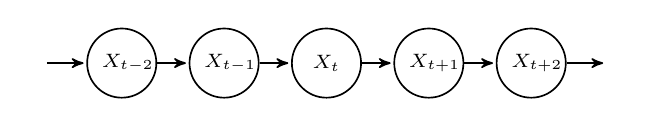
\begin{tikzpicture}[->,>=stealth',shorten >=1pt,auto,node distance=1.3cm,
                    semithick, baseline=1em]
	  \tikzstyle{every state}=[fill=white,draw=black,text=black,text width=0.5cm, align=center]

	  \node[state] 		   (x-2)                    	{\scriptsize$X_{t-2}$};
	  \node[state]         (x-1) [right of=x-2] 		{\scriptsize$X_{t-1}$};
	  \node[state]         (x) [right of=x-1] 		{\scriptsize$X_{t}$};

	  \node[state]         (x1) [right of=x] 		{\scriptsize$X_{t+1}$};
	  \node[state]         (x2) [right of=x1]       {\scriptsize$X_{t+2}$};

	  \node[text width=0pt]			(start) [left=0.5cm of x-2] {};
	  \node[text width=0pt]			(end) [right=0.5cm of x2] {};

	  \path (start) edge (x-2)
	  (x-2) edge (x-1)
	  (x-1) edge (x)
	  (x) edge (x1)
	  (x1) edge (x2)
	  (x2) edge (end);
	\end{tikzpicture}
\end{center}
\vspace{1em}
Markovprozess zweiter Ordnung
\vspace{1em}
\noindent
\begin{center}
	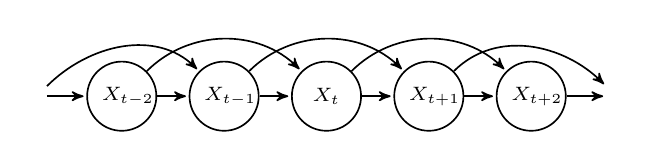
\begin{tikzpicture}[->,>=stealth',shorten >=1pt,auto,node distance=1.3cm,
                    semithick, baseline=1em]
	  \tikzstyle{every state}=[fill=white,draw=black,text=black,text width=0.5cm, align=center]

	  \node[state] 		   (x-2)                    	{\scriptsize$X_{t-2}$};
	  \node[state]         (x-1) [right of=x-2] 		{\scriptsize$X_{t-1}$};
	  \node[state]         (x) [right of=x-1] 		{\scriptsize$X_{t}$};

	  \node[state]         (x1) [right of=x] 		{\scriptsize$X_{t+1}$};
	  \node[state]         (x2) [right of=x1]       {\scriptsize$X_{t+2}$};

	  \node[text width=0pt]			(start) [left=0.5cm of x-2] {};
	  \node[text width=0pt]			(end) [right=0.5cm of x2] {};

	  \path (start) edge (x-2) edge[in=135, out=45] (x-1)
	  (x-2) edge (x-1) edge[in=135, out=45] (x)
	  (x-1) edge (x) edge[in=135, out=45] (x1)
	  (x) edge (x1) edge[in=135, out=45] (x2)
	  (x1) edge (x2) edge[in=135, out=45] (end)
	  (x2) edge (end);
	\end{tikzpicture}
\end{center}
\vspace{1em}




\begin{itemize}
	\item Markov Prozesse
	\item Hidden Markov Models
\end{itemize}


\section{Neuronale Netze}
\subsection{Graphische Repräsentationen}


\section{Erklärbarkeit von Entscheidungen}







\section{unassigned}
\begin{itemize}
	\item Belief Space Planning for Bandits 07/22ff
\end{itemize}
\end{document}
